\chapter{Introducción}

Este documento presenta los apuntes realizados del libro \textit{Machine Learning for Text} con  ISBN 978-3-319-73531-3 (eBook, 2018) de Charu C. Aggarwal un distinguido investigador de IBM; El motivo de redactar este documento es aprender sobre el procesamiento del lenguaje natural para ser aplicado en el trabajo terminal (TT) \textbf{Recolector y clasificador de noticias} con número 2019-B013, de la \textbf{Escuela superior de cómputo} (ESCOM) del \textbf{Instituto politécnico nacional} (IPN).\\

\section{Machine learning for text}

La extracción de información útil con varios tipos de algoritmos estadísticos es denominado \textbf{Extracción de datos}( \textit{Text mining} ), \textbf{Analítica de texto} (\textit{Text analytics}) o \textbf{Aprendizaje automático para texto} (\textit{Machine learning for text}), en este documento se utilizará de forma indistinta. En los últimos años este campo ha incrementado por el desarrollo de la web, redes sociales, correos electrónicos, bibliotecas virtuales. Algunos ejemplos para obtener información son:

\begin{itemize}

	\item \textbf{Bibliotecas digitales}: El uso de la información electrónica ha superado la producción de libros y publicaciones impresas, este fenómeno ha proliferado la producción de bibliotecas digitales, estas pueden ser almacenadas y ser usadas para extraer información útil.

	\item \textbf{Noticias electrónicas}: Existe un movimiento masivo para pasar las noticias impresas hacía la publicación electrónica, esto permite que sean almacenadas para su análisis y extracción de información sobre eventos y perspectivas importantes. Sitios como \textit{Google news} etiquen las noticias para hacer recomendaciones al lector basado en su anterior comportamiento o intereses específicos.

	\item \textbf{\textit{Web and Web-enabled applications}}: La web contiene una gran cantidad de información en hipertexto, con links y otro tipo de recursos, la cual puede ser utilizada par el proceso de descubrimiento de nuevo conocimiento, al igual las \textit{Web-enabled applications}\footnote{\textbf{\textit{Web and Web-enabled applications}}: Aplicaciones de escritorio que son  accedidas remotamente des de un buscador como Internet explorer.} permiten obtener información que puede ser analizada.

	\item \textbf{Redes sociales}: Las redes sociales son un campo que está proliferando, debido a su naturaleza donde cada usuario contribuye con sus propias publicaciones.

\end{itemize}



Algunas de las aplicaciones son las siguientes:

\begin{itemize}

	\item Etiquetar la web, permite al usuario encontrar paginas de interés

	\item Los proveedores de correos, utilizan la información almacenada para mostrar publicidad de interés al usuario

	\item Algunas páginas ordenan su contenido de acuerdo a su importancia

	\item El análisis de las opiniones es un campo de importancia así como el análisis de sentimientos		

\end{itemize}


El orden se las palabras en un texto brindan un significado semántica el cual no puede ser inferido  solo con la frecuencia de las palabras. Sin embargo, se pueden hacer varias predicciones sin contemplar la semántica. Existen 2 tipos de representaciones que son populares en las aplicaciones de \textbf{text mining}:

\begin{itemize}
	
	\item \textbf{\textit{Text as a bag-of-words}}: Es la representación mas común. No se contempla el orden de las palabras el proceso. El conjunto de palabras en el documento se convierten en \textit{Sparse multidimentional reprentation}, el cual corresponde a la dimensión en esta representación. Se utiliza para la clasificación, sistemas de recomendación.

	\item \textbf{\textit{Text as a set of sequences}}: En esta representación se extraen sentencias, el orden de las palabras si importa. La unidad son sentencia o párrafos. Es utilizado en aplicaciones que necesitan un fuerte uzo de la semántica, esta área se acerca mucho al modelado de lenguaje y procesamiento del lenguaje natural

\end{itemize}


\section{Definiciones}

\subsection{Corpus}

En el desarrollo de las aplicaciones se tiene un conjunto de datos los cuales forman el \textit{corpus}, el orden de los datos se coloca en $10^5$ es decir 100,000 datos o incluso $10^6$. En la mayoría de los datos toman el valor de 0, solo un pequeño conjunto toma un valor positivo.

\subsection{Learning algorithm}

El término \textit{Learning algorithm} se utilizará para hacer referencia a los algoritmos que descubran patrones en el texto, o como se pueden usar los patrones para predecir valores específicos en los datos.


\section[Pre-procesamiento]{Pre-procesamiento y computación similar}

El Pre-procesamiento es necesario para convertir el formato no estructurado en un formato estructurado.
A menudo el texto contiene información extraña como etiquetas, \textit{anchor text}\footnote{Es el texto mostrado en los enlaces o hipervínculos, \textbf{Texto de anclaje} en español.}, y otras características. En muchos casos las palabras son variaciones de otras (Sinónimos) por el tipo de redacción, el contexto, para eliminar redundancia. Algunas palabras simplemente tienen faltas de ortografía. El proceso de convertir una secuencia de caracteres en una secuencia de palabras(Tokens), es llamado \textbf{Tokenización}. Además por cada palabra repetida se crea un token, es decir al repetirse una palabra 3 veces, se crearán 3 tokens correspondientes. Alguno de los pasos mas comunes para el procesamiento de texto en bruto son los siguientes: 

\begin{itemize}

	\item \textbf{Extracción de texto}: En caso de recuperar información de la web, se tiene que limpiar el texto ya que contiene \textit{anchor text}, etiquetas.Se debe buscar los bloques que brinden información útil para el análisis, ya que algunos bloques contienen publicidad o información no relacionada. Para esto se tiene que realizar un \textbf{parseo}\footnote{Es la acción de analizar el texto de forma especializada} o técnicas de extracción especializadas.

	\item \textbf{Remover stop-words}: \textbf{Stop words}, son pronombres, \textit{articles} y preposiciones que deben ser removidas para mejorar la compresión del texto.

	\item  \textbf{Stemming, case-folding, punctuation}: Las palabras que derivan de la misma raíz como hundimiento, se hundió, se reducen a hundir. Una palabra puede tener diferentes significados dependiendo el contexto como la palabra \'Rosa\' puede hacer referencia a una flor o el nombre de una persona, por lo tanto se requiero la euristica del lenguaje específico para poder tomar una decisión en como debe ser interpretada. Los signos de puntuación como el guión medio deben ser tratados con mucho cuidado para realizar una buena tokenización.

	\item \textbf{\textit{Frequency-based normalization}}: Palabras con poca frecuencia son mas discriminatorias que las de alta frecuencia. Por lo tanto se pondera la importancia de los documentos con base al calculo de la \textbf{frecuencia inversa del documento}(\textit{fid}) en la colección. Si $\psi_i$ es el número de documentos en el cual la palabra aparece, y $\psi$ es el número total de documentos, la \textit{fid} se calcula como $log(\frac{\psi}{\psi_i})$. La importancia de un documento se calcula multiplicando la \textbf{frecuencia de término} (\textit{ft}) en el documento por la \textit{fid}. Mientras la \textit{ft} brinda la cantidad de veces  que una palabra aparece en el documento la \textit{fid} especifica la importancia en la colección; Se define como \textbf{ft-fid} o \textit{tf-idf} (Por su sigla en ingles \textit{Term frequency – Inverse document frequency}). La figura \ref{fig:G1-ln} muestra como en proporción a la aparición baja de la palabra  en los documentos gana un valor superior (Es decir gana importancia); La figura \ref{fig:G2-x} muestra como una palabra gana importancia al tener una frecuencia alta en el documento.

	\begin{figure}[h]
	\centering
	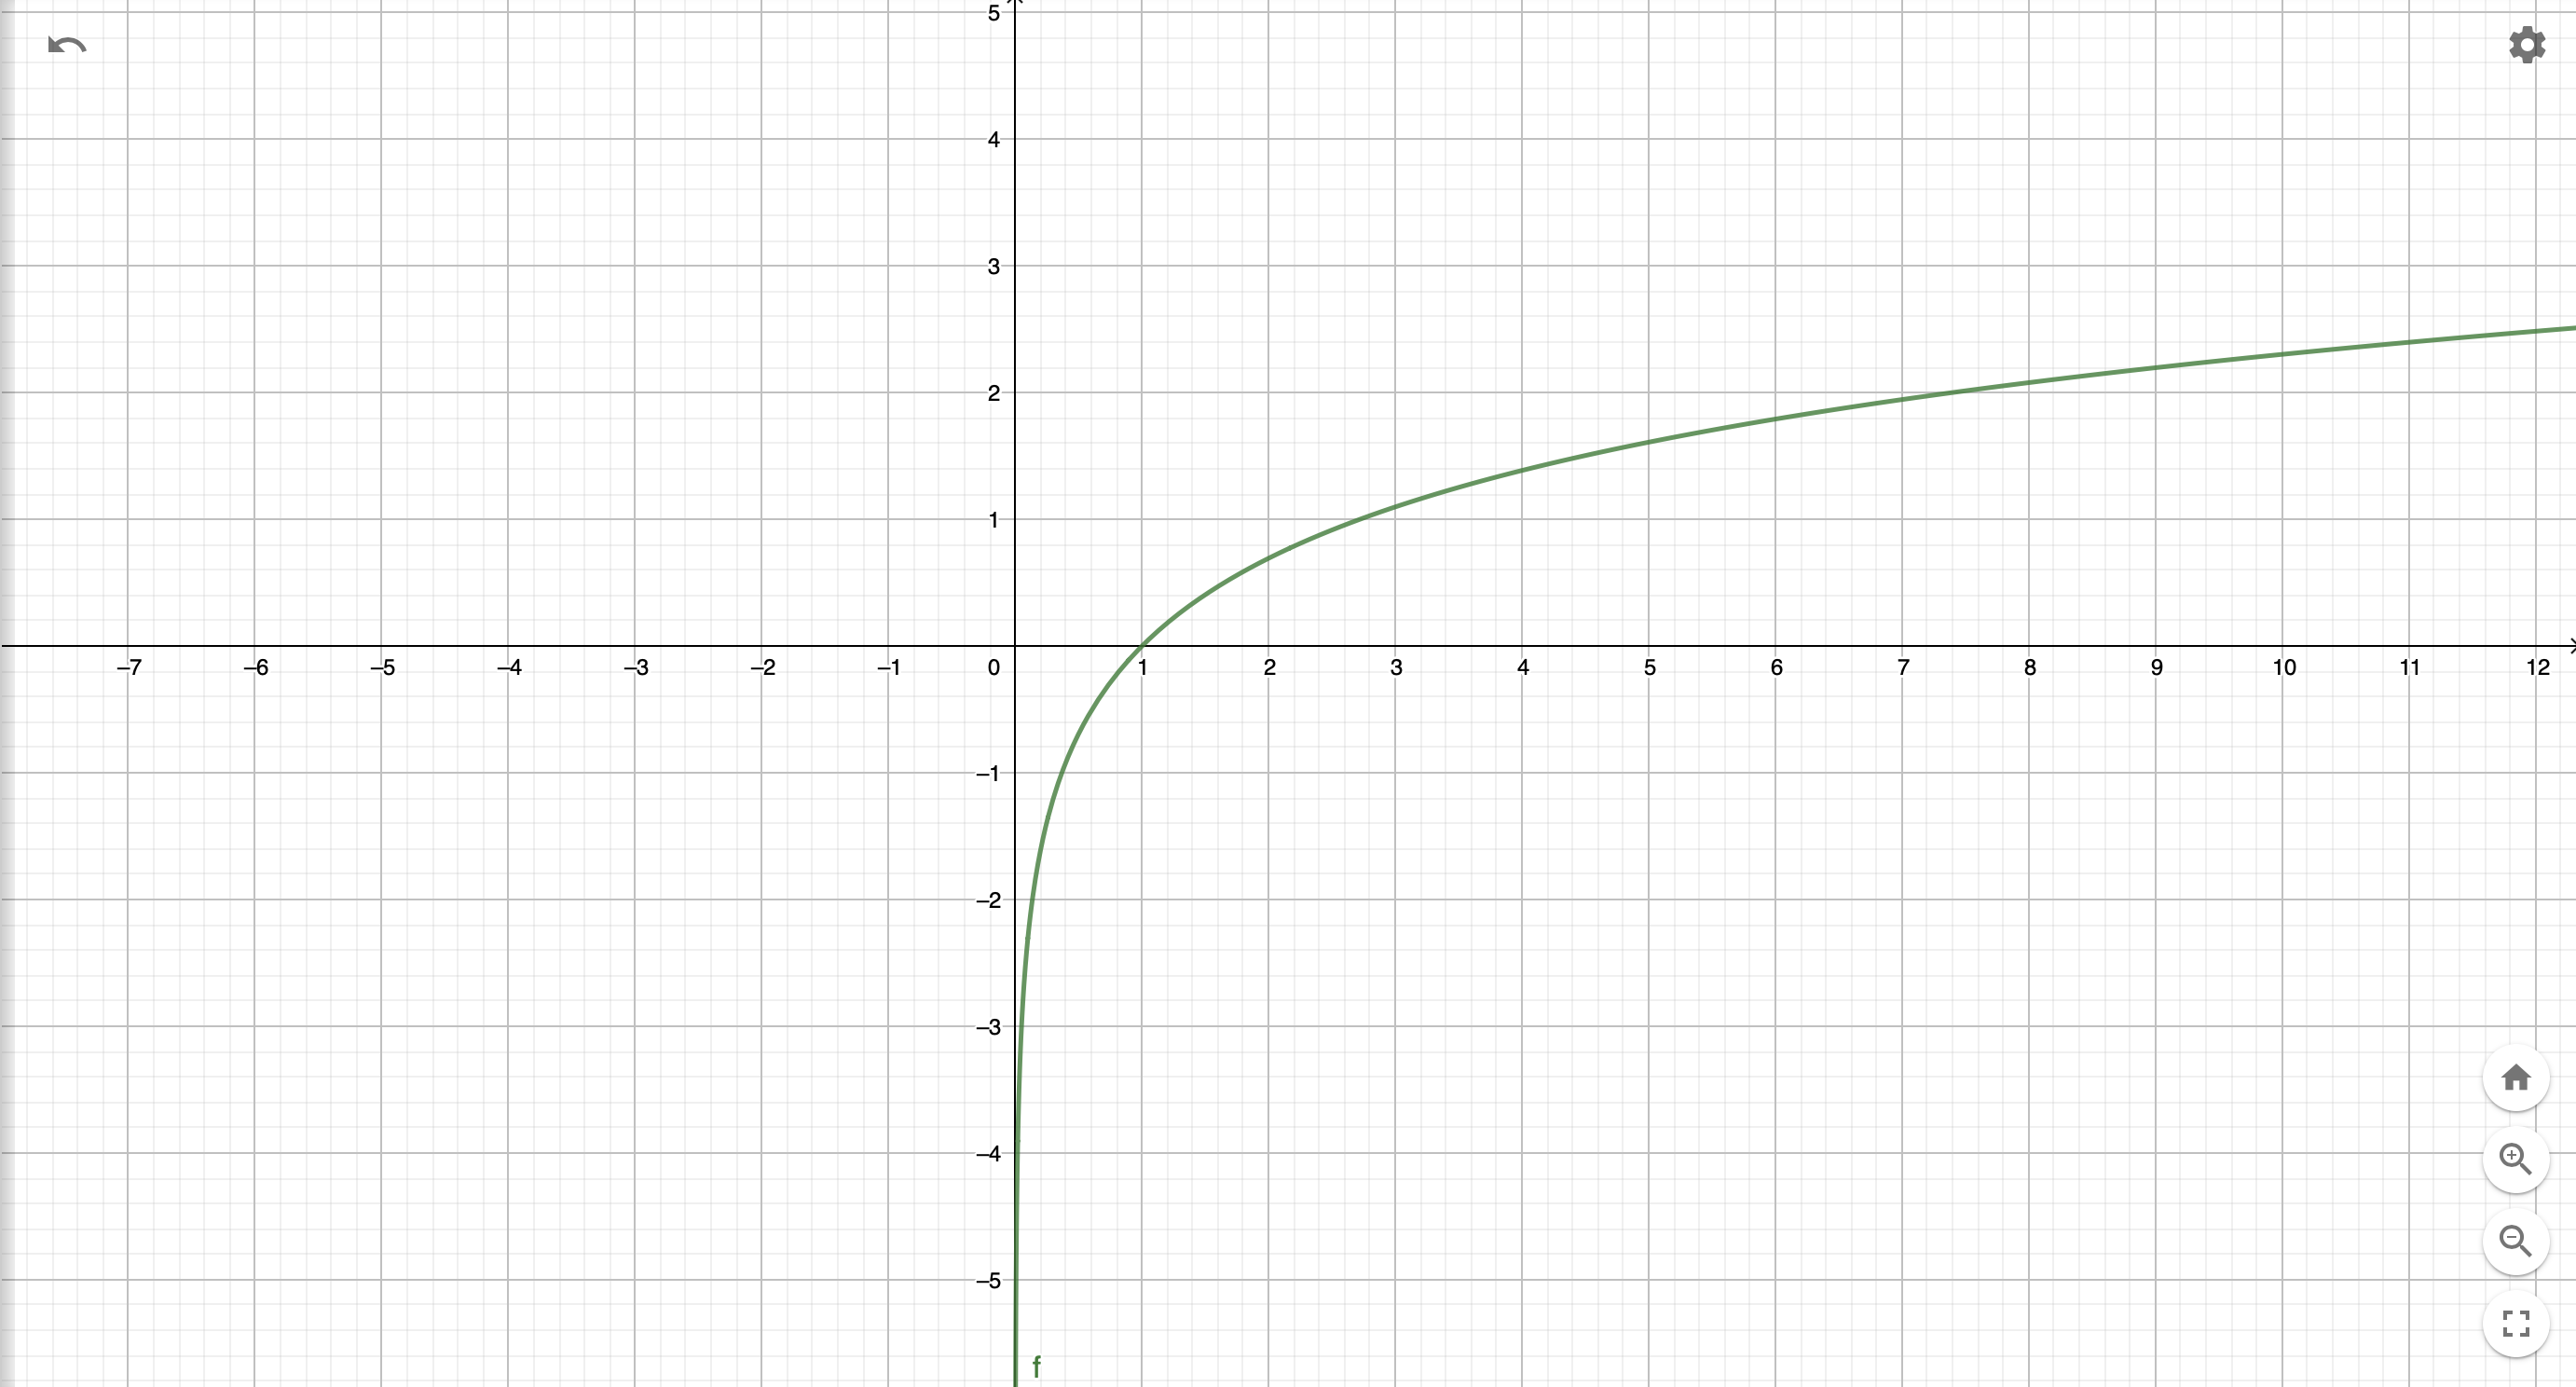
\includegraphics[scale=.2]{Imagenes/ln.png}	
	\caption{Gráfica \textit{Inverese document frequency}}
	\label{fig:G1-ln}
	\end{figure}


	\begin{figure}[h]
	\centering
	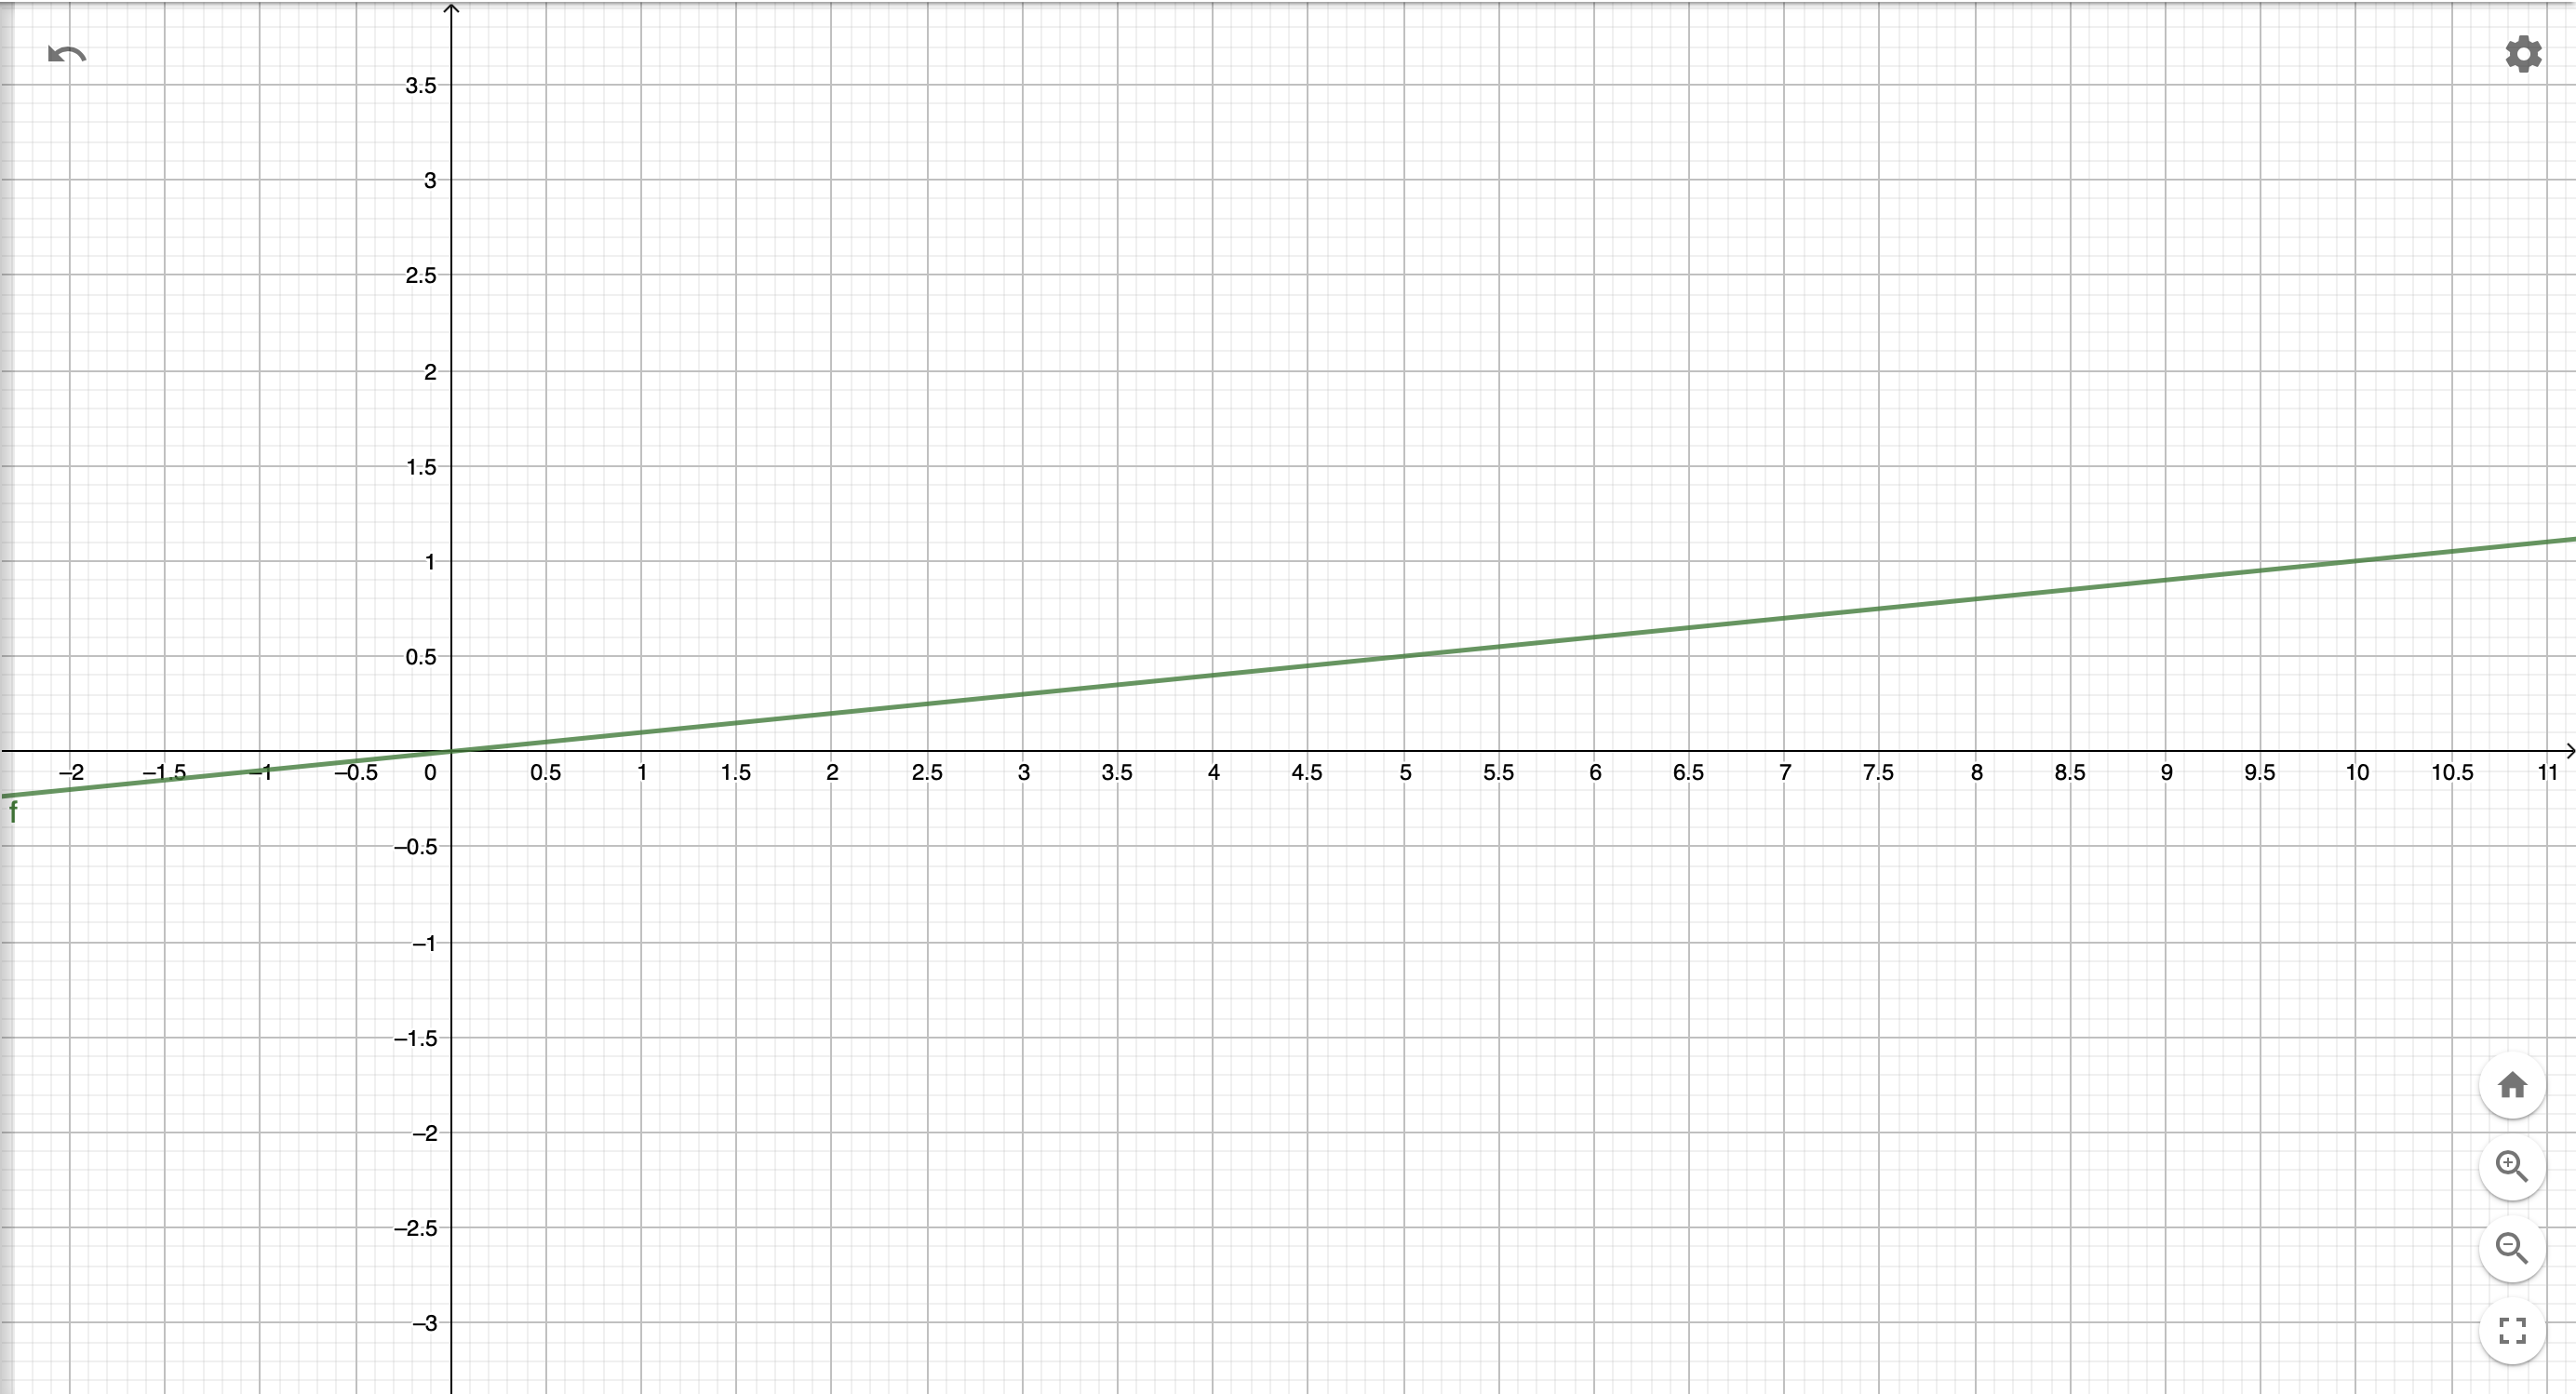
\includegraphics[scale=.2]{Imagenes/x_10.png}
	\caption{Gráfica de \textit{Term frequency}}
	\label{fig:G2-x}
	\end{figure}	




\end{itemize}